\chapter{Finishing Decode}

\section{iDecode Module}
At this point, you have created all of the modules necessary to assemble the iDecode module.  Now you need to create a new module called iDecode.  The inputs and outputs can be determined by evaluating Figure~\ref{fig:decode_stage}.  Any signal that crosses the boundaries of the red box is an input or output.  Signals that do not cross the boundaries of the red box are signals that are internal to the iDecode module and should be declared internally in iDecode, with the exception of reg\_write and reg2\_loc.  reg\_write and reg2\_loc should be declared as output signals.  This will help when we pipeline the datapath later in the semester.   Please make sure to label signals consistently with lower case letters with words separated by underscores.  For example, read\_data1, write\_data, alu\_src.  

Also, make sure to use the instr\_parse module in iDecode.  iDecode.v should not use any signals that specify particular bits to use.  For instance, for the read\_register1 input port on the regfile module, you should connect the rn\_num signal from the instr\_parse module rather than using something instruction[9:5].  

\begin{figure}
	\caption{Expected Results}\label{fig:decode_stage}
	\begin{center}
		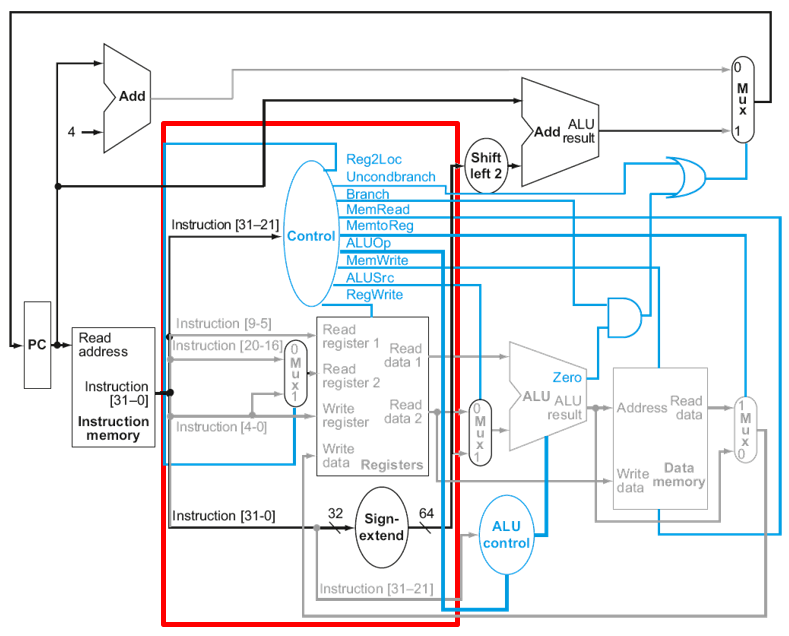
\includegraphics[width=4.75in]{../images/decode_stage.png}
	\end{center}
\end{figure} 


\section{iDecode Testbench}
To verify that your iDecode module works correctly, you must first fill in the Expected Results Table (Lab6\_ExpectedResultsTable.xlsx) that has been provided in the tables directory. All rows and columns have been defined, but you must fill the expected values into each cell.  If a particular data item is not relevant for a particular instruction (for instance, sign\_extended\_output on an R-type instruction), then put N/A in that cell.  It is important that we identify which signals are applicable and which signals are not applicable.  Please do not use N/A for any control signals, as we always want to make sure these are set correctly.  

To ensure that we are testing each case correctly and consistently, please update regData.data to reflect the following values and use these values when making filling in your Expected Results Table.  Note that the instructions execute, so if X9 is updated by the first instruction, then you should use the updated value of X9 in the second instruction, etc.  However, we will not be branching at this time, so the instructions will run in order.

\begin{enumerate}
	\item X19 = 10
	\item X20 = 30
	\item X21 = 0
	\item X22 = 16
\end{enumerate}

Now update the provided testbench for iDecode to provide the inputs for iDecode and verifying the outputs of iDecode.  For the instruction input, use the instructions from your Expected Results Table.  For the outputs, use your Expected Results Table to fill in the 'er' values for each instruction.  For instructions that update the register file, use the test bench to provide the correct value to the write\_data input, since we do not yet have an ALU to do the calculations or memory to load from.  Please use your test bench to provide a value of 20 to X9 in the first command (LDUR).

In the testbench, when there is a value that is N/A in your Expected Results Table, please comment out the verify function call for that signal, since we do not have a real expected result to compare it to.  Doing this, the testbench should end up having 119 test cases.

\section{Your Assignment}

You are to:
\begin{enumerate}
\item Integrate all individual modules into the iDecode module.
\item Update your Expected Results Table to include values for all iDecode inputs and outputs.
\item Update iDecode\_test.sv with values from the Expected Results Table.  Note that you should not add any test cases, change timing, etc.
\item Verify that your simulation results match your expected results.
\item Rather than writing a lab report, please produce a landscape mode PDF file called Lab6\_lastname.pdf that includes (in this order):
\begin{enumerate}
	\item Your name and the lab number.
	\item A snip of your completed Expected Results Table.
	\item A snip of the Simulation Results for the iDecode module.  Please show instructions in hex, opcodes and control signals in binary and everything else in signed decimal.  
	\item A snip of the test results from the Tcl Console for the iDecode module.  This snip should show the entire log from BEGIN TEST RESULTS to END TEST RESULTS.	
\end{enumerate}
\item Upload Lab6\_lastname.pdf file to Canvas.
\item Zip up your ARM-Lab directory and submit it on Canvas as well.  Please make sure that you give me the ARM-Lab directory rather than the ARM-Project directory.  I do not want the project files in the ARM-Project directory.  Before you submit your zip file, extract the file and make sure that the top-level directory is called ARM-Lab and that the lower level directories like code, manual, etc are directly beneath ARM-Lab in the directory structure.  I will extract your zip file and run your code against my correct testbench to verify that your code and testbench work correctly, and it is critical that everyone's directory structure is consistent.
\end{enumerate} 